% !TeX spellcheck = de_DE
\documentclass[a4paper, 12pt]{article}

\usepackage{bm, bbm, wrapfig, float, setspace, amsmath, amssymb, amsthm, url, graphicx, ngerman, transparent, enumerate, bbold, esint, polynom, hyperref, microtype, etoolbox, braket, cleveref, hyphenat, stmaryrd}
\usepackage{centernot}

\usepackage{tikz}
\usepackage{epsdice}
\usepackage{listings}
\lstset{language=Python}
\tikzset{>=stealth}
\usetikzlibrary{decorations.markings, shapes, calc}

\renewcommand{\familydefault}{cmss}   % Generates sans serif fonts


\renewcommand{\l}{\left(}
\renewcommand{\r}{\right)}
\newcommand{\gs}{\text{gs}}
\renewcommand{\P}{\hat{P}}
\newcommand{\U}{\hat{U}}

% \newcommand{\bra}[1]{\langle#1|}
% \newcommand{\ket}[1]{|#1\rangle}
\newcommand{\bkt}[2]{\left\langle #1 |#2 \right\rangle}
\renewcommand{\ij}{{\langle \vec{i}, \vec{j} \rangle}}
\renewcommand{\H}{\hat{\mathcal{H}}}
\newcommand{\Ht}{\tilde{\mathcal{H}}}
\renewcommand{\c}{\hat{c}}
\renewcommand{\a}{\hat{a}}
\newcommand{\cd}{\hat{c}^\dagger}
\newcommand{\rh}{\hat{\rho}}
\newcommand{\rht}{\tilde{\rho}}
\newcommand{\ad}{\hat{a}^\dagger}
\newcommand{\bd}{\hat{b}^\dagger}
\newcommand{\ubd}{\hat{\uline{b}}^\dagger}
\newcommand{\ub}{\hat{\uline{b}}}
\renewcommand{\b}{\hat{b}}
\newcommand{\hd}{\hat{h}^\dagger}
\newcommand{\h}{\hat{h}}
\renewcommand{\d}{\hat{d}}
\newcommand{\n}{\hat{n}}
\newcommand{\D}{\hat{D}}
\newcommand{\Dd}{\hat{D}^\dagger~\hspace{-0.12cm}}

\newcommand{\G}{\hat{\Gamma}}
\newcommand{\Gd}{\hat{\Gamma}^\dagger}
\newcommand{\F}{\hat{F}}
\newcommand{\Fd}{\hat{F}^\dagger}
\newcommand{\hc}{\text{h.c.}}
\newcommand{\MF}{\text{MF}}
\newcommand{\BEC}{\text{BEC}}
\newcommand{\RG}{\text{RG}}
\newcommand{\psd}{\hat{\psi}^\dagger}
\newcommand{\ps}{\hat{\psi}}
\newcommand{\I}{\text{I}}
\newcommand{\p}{\text{p}}
\newcommand{\f}{\text{F}}
\newcommand{\s}{\text{S}}
\renewcommand{\sf}{\text{MIX}}
\renewcommand{\O}{\hat{\mathcal{O}}}
\newcommand{\W}{\hat{W}}
\newcommand{\Ud}{\hat{U}^\dagger}
\newcommand{\HMF}{\mathscr{H}_{\text{MF}}}
\newcommand{\ph}{\text{ph}}
\newcommand{\IB}{\text{IB}}
\newcommand{\B}{\text{B}}
\newcommand{\eff}{\text{eff}}
\newcommand{\tr}{\text{tr}}
\newcommand{\tdiff}{\,\mathrm{d}}
\newcommand{\nodagger}{{\vphantom{\dagger}}}
 % \newcommand{\longmapsfrom}{\longleftarrow\!\shortmid}

\normalsize
\setlength{\hoffset}{-1.5cm}
\addtolength{\textwidth}{3cm}
\setlength{\voffset}{-2.2cm}
\addtolength{\textheight}{3.5cm}
\addtolength{\footskip}{0.2cm}

%\input{macros.tex}
\newtheorem{aufgabe}{Problem}
\newtheorem{bspaufgabe}{Beispielaufgabe}

\usepackage{titlesec}

\titleformat{\section}[block]
{\normalfont}{\textbf{Problem \thesection}}{1em}{}

\DeclareMathOperator{\dd}{d}
\newcommand{\eul}{\text{e}}

% imaginary unit 
\newcommand{\imag}{\textsl{i}}
%
% with or without solution?
%
\makeatletter
\@ifundefined{solfalse}{
\newif\ifsol
\soltrue
}
\makeatother
\newcommand{\solA}{\vskip0.5em \color{brown}\noindent\textbf{Solution:\\}}
\newcommand{\sol}[1]{\vskip0.5em \color{brown}\noindent\textbf{Solution:}\\#1}

\usepackage{relsize}
\newcommand\Cpp{C\nolinebreak[4]\hspace{-.05em}\raisebox{.4ex}{\relsize{-3}{\textbf{++}}}}

\begin{document}
	   
% ********** First Box **************
\vspace*{-13mm}
\noindent\fbox{
	\parbox[b][19mm][b]{16mm}{%\parbox[POS][H�HE][POS-INNEN]{BREITE}{INHALT}
		\center
\includegraphics[trim=1.6mm  0 0 0, width=18mm]{../../images/lmu-bildmarke.png}
	}
}
\hfill
% ********** Second Box **************
% Diese Schrift sollte so gross sein, dass die Oberkante des Ms von
% Max mit der Oberkante von LMU abschliesst
\fbox{\parbox[b][19mm][b]{19mm}{
\includegraphics[width=19mm,height=19mm]{../../images/lmu-wortmarke.png}}}%
\hfill\hfill
% ********** Third Box **************
\fbox{\parbox[b][19mm][b]{84mm}{\fontsize{9}{12}\sc Faculty of Physics, Summer Term 2023 \\  Numerical Quantum Physics\\ 
		Lecturer: Dr. S. Paeckel \\ Assistant Lecturer: Z. Xie, B. Schneider
		\vspace{0.1mm}}}
\hfill
% ********** Fourth Box **************
\fbox{
	\parbox[b][19mm][b]{25mm}{\hspace*{3mm}\transparent{0.52}{\vspace{-1mm}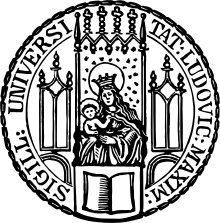
\includegraphics[trim=0 6mm 16mm 20mm, clip, height=21mm]{../../images/lmu-siegel.png}}\transparent{1}}
}
\begin{center}
	\small \url{https://www2.physik.uni-muenchen.de/lehre/vorlesungen/sose_23/nqp/}
\end{center}
%
\vspace{8mm}
%
\centerline{\Large\textbf{Sheet~3:~Matrix-product states}}
%
\vspace{3mm}
%
\normalsize\centerline{Released:~05/19/23;~Submit until:~06/09/23 (\textbf{20 Points})}
%
%\vspace{0mm}
%
%
\vspace{6mm}
%
Matrix-product states (MPS) are maybe the most successful framework for studying one-dimensional systems.
%
In the following, we will set up a small toolkit that implements the an important property of MPS: The compression of wave functions.
%
To achieve that goal, we need a few ingredients that allow us to work with rank-$3$ tensors, which are at the heart of representing wave functions as MPS.
%

%
\section{Fusing and splitting \textbf{(4 Points)}}
%
Consider a set of rectangular matrices $\mathbf{M}^k\in \mathbb V_{\mathbb K}^{m\times n}$ ($\mathbb K = \mathbb R, \mathbb C$) where $k\in \left\{ 0,\ldots,d-1 \right\}$ for some $d\in\mathbb N$.
%
Writing for each $k$ the matrices component-wise $M^k_{\alpha, \beta}$, we define a left (right) fusion by merging the index $k$ with the index $\alpha$ ($\beta$):
\begin{equation}
	\text{Left fusion: } M_{(k,\alpha), \beta} \in \mathbb V_{\mathbb K}^{d\cdot m \times n} \;, \quad
	\text{Right fusion: } M_{\alpha, (k,\beta)} \in \mathbb V_{\mathbb K}^{m \times d\cdot n} \; .
\end{equation}
%
The fused indices are mapped to a new index via $(k,\alpha) = k\cdot m + \alpha$ and $(k,\beta) = k\cdot n + \beta$ and can be realized by stacking the matrices $M^k$ either vertically, or horizontally.
%
Similarly, we define the left (right) splitting by decomposing the fused indices
\begin{align}
	\text{Left splitting: } &k = (k,\alpha) \operatorname{div} m\;, &\alpha &= (k,\alpha) \operatorname{mod} m \\
	\text{Right splitting: } &k = (k,\beta) \operatorname{div} n\;, &\beta &= (k,\beta) \operatorname{mod} n \; ,
\end{align}
where $\operatorname{div}$ denotes the integer division and $\operatorname{mod}$ the modulo operation.
%
For both operations of index fusing and splitting, write two functions performing the left and write fusing and splitting.
%
For the fusion operation, the functions map a set of matrices to a bigger matrix: $ M^k_{\alpha, \beta} \longmapsto M_{(k,\alpha), \beta}$.
%
For the splitting operation, the functions map a big matrix into a set of smaller matrices: $ M_{(k,\alpha), \beta} \longmapsto M^k_{\alpha, \beta}$.
%
Write reasonable test cases to ensure the correct functionality of your implementations.
%

%
\section{Matrix-product states and the canonical form \textbf{(8 Points)}}
%
A matrix-product state is simply a collection of sets of matrices (rank-$3$ tensors) that is, to each lattice site we are assigning such a set $M^{k_j}_{\alpha_{j-1}, \alpha_{j}}$.
%
Note that the index $j\in\left\{0, \ldots, L-1\right\}$ is introduced to label the different matrix dimensions $\alpha_j, \alpha_j$ and matrices $k_j$ at the different sites and $L$ denotes the number of lattice sites.
%
Such a matrix-product state allows to represent the coefficients of a wave function $c_{k_0, k_1, \ldots, k_{L-1}} \in\mathbb K$ on a tensor-product Hilbert space:
\begin{equation}
	\ket{\psi(\left\{\mathbf M^{k_j}\right\})} = \sum_{k_0,\ldots,k_{L-1}} \underbrace{\mathbf M^{k_0} \cdot \mathbf M^{k_1} \cdots \mathbf M^{k_{L-1}}}_{c_{k_0, k_1, \ldots, k_{L-1}}} \ket{n_{k_0}, \ldots, n_{k_{L-1}}} \; ,
\end{equation}
where $\ket{n_{k_j}}$ are the basis states of the $j$th degress of freedom.
%
In particular, for spin systems we have $d=2$ with $\ket{n_{k_j=0} = \downarrow}$ and $\ket{n_{k_j=1} = \uparrow}$.
%
\begin{itemize}
	\item[(2.a)] \textbf{(3P)}
	%
	Implement a class \texttt{MPS} that contains a collection of $L$ such sets of matrices $M^{k_j}_{\alpha_{j-1}, \alpha_{j}}$.
	%
	These matrices should have dimensions $m_j \leq m$ and we will call $m\in\mathbb N$ the maximum bond dimension.
	%
	Note that at the ends of the MPS, i.e., $j=0$ and $j=L-1$, the matrix dimensions have to be such that the overall MPS contracts to a number: $\alpha_0 = \alpha_L \equiv 1$.
	%
	The parameter $m$ should be a property of the MPS class.
	%
	Also write a method that initializes the set of site matrices either via input parameters, or with random numbers.
	%
	\item[(2.b)] \textbf{(5P)}
	%
	In order to perform numerical optimizations we use the canonical form.
	%
	It is defined by fixing the additional gauge degrees of freedom of the MPS-representation via:
	\begin{align}
		\text{Left orthogonal: } &\sum_{(k_j,\alpha_{j-1})} M^\dagger_{(k_j,\alpha_{j-1}),\alpha_j} M^\nodagger_{(k_j,\alpha_{j-1}),\beta^\prime_j} = \delta_{\alpha_j,\alpha^\prime_j} \\
		\text{Right orthogonal: } &\sum_{(k_j,\alpha_{j})} M^\nodagger_{\alpha_{j-1},(k_j,\alpha_j)} M^\dagger_{\alpha^\prime_{j-1},(k_j,\alpha_j)} = \delta_{\alpha_{j-1},\alpha^\prime_{j-1}}
	\end{align}
	%
	Note that these conditions can be evaluated easily as matrix-matrix product of left-/right-fused matrices.
	%
	In practice, we fix the gauge by performing a singular value decomposition (SVD) of the left-/right-fused matrices
	\begin{align}
		\text{Left orthogonal: } &M_{(k_j,\alpha_{j-1}),\alpha_j} = \sum_{s_j} U_{(k_j,\alpha_{j-1}),s} S_{s_j} V_{s_j,\alpha_j} \;, \\
		\text{Right orthogonal: } &M_{\alpha_{j-1},(k,\alpha_j)} = \sum_{s_j} U_{\alpha_{j-1},s_j} S_{s_j} V_{s_j,(k,\alpha_j)} \;.
	\end{align}
	%
	For each gauge, implement a function which performs an SVD on the fused matrices of a given site.
	%
	For the left orthogonal gauge, replace the set of site matrices with the set of splitted $U$-matrices: $M^{k_j}_{\alpha_{j-1},\alpha_j} \longmapsfrom U^{k_j}_{\alpha_{j-1},s_j}$ and multiply the remainder of the SVD to the set of site matrices to the right: $M^{k_{j+1}}_{\alpha_j,\alpha_{j+1}} \longmapsfrom \sum_{\alpha_{j}} S_{s_j} V_{s_j,\alpha_j} M^{k_{j+1}}_{\alpha_j,\alpha_{j+1}}$.
	%
	Accordingly, for the right orthogonal gauge, replace the set of site matrices with the set of splitted $V$-matrices: $M^{k_j}_{\alpha_{j-1},\alpha_j} \longmapsfrom V^{k_j}_{s_j, \alpha_{j}}$ and multiply the remainder of the SVD to the set of site matrices to the left: $M^{k_{j-1}}_{\alpha_{j-2},\alpha_{j-1}} \longmapsfrom \sum_{\alpha_{j-1}} M^{k_{j-1}}_{\alpha_{j-2},\alpha_{j-1}} U_{\alpha_{j-1},s_j} S_{s_j}$.
	%
\end{itemize}
%
Don't forget to write test cases that ensure the correct orthogonality properties of the set of site matrices.
%

%
\section{Compression of wave functions \textbf{(8 Points)}}
%
The canonical form can be used to efficiently represent quantum-many body states by maximizing the overlap between a guess state $\ket{\tilde \psi}$ and the target state $\ket{\psi}$.
%
In order to simplify the notation, we denote those sets of site matrices satisfying the left-orthogonal condition by $\mathbf A^{k_j}$ and those satisfying the right-orthogonal condition by $\mathbf B^{k_{j}}$.
%
We furthermore denote the left fusion of a set of site-matrices by adding an arrow to the left: $\overset{\shortleftarrow}{\mathbf M}_j$ and correspondingly denote the right fusion of a set of site matrices by adding an arrow to the right: $\overset{\shortrightarrow}{\mathbf M}_j$.
%
Note that using that notation we have $\overset{\shortleftarrow}{\mathbf A}_j^\dagger = \overset{\shortrightarrow}{\mathbf A}^*_j$ and $\overset{\shortrightarrow}{\mathbf B}_j^\dagger = \overset{\shortleftarrow}{\mathbf B}^*_j$ where the star denotes the adjoint matrix, as well as:
\begin{equation}
	\overset{\shortrightarrow}{\mathbf A}^*_j \overset{\shortleftarrow}{\mathbf A}_j = \mathbb 1_{m_j \times m_j} \quad \text{and} \quad
	\overset{\shortrightarrow}{\mathbf B}_j \overset{\shortleftarrow}{\mathbf B}^*_j = \mathbb 1_{m_{j-1} \times m_{j-1}} \; .
\end{equation}
%
Finally, we define the mixed-canonical form of a wave function with gauge-center $j$ via
\begin{equation}
	\ket{\psi(j)} = \sum_{k_0,\ldots,k_{L-1}} \mathbf A^{k_0} \cdots \mathbf A^{k_{j-1}} \mathbf M^{k_j} \mathbf B^{k_{j+1}} \cdots \mathbf B^{k_{L-1}} \ket{n_{k_0}, \ldots, n_{k_{L-1}}} \; .
\end{equation}
%
We can therefore write the overlap between two states $\ket{\psi}, \ket{\tilde \psi}$ as
\begin{equation}
	\braket{\tilde \psi | \psi}
	=
	\operatorname{Tr} \sum_{k_j}  \left(\tilde{\mathbf M}^{k_j}\right)^\dagger \overset{\shortrightarrow}{\tilde{\mathbf A}}^*_{j-1} \cdots \overset{\shortrightarrow}{\tilde{\mathbf A}}^*_{0} \overset{\shortleftarrow}{\mathbf A}_{0} \cdots \overset{\shortleftarrow}{\mathbf A}_{j-1} \mathbf M^{k_j} \overset{\shortrightarrow}{\mathbf{B}}_{j+1} \cdots \overset{\shortrightarrow}{\mathbf{B}}_{L-1}\overset{\shortleftarrow}{\tilde{\mathbf{B}}}^*_{L-1} \cdots \overset{\shortleftarrow}{\tilde{\mathbf{B}}}^*_{j+1}  \; ,
\end{equation}
where fused matrix sets with a tilde belong to the state $\ket{\tilde \psi}$.
%
Optimization of the cost function $\lVert \ket{\psi} - \ket{\tilde{\psi}}\rVert$ with respect to the coefficients $\tilde{M}^{k_j}_{\alpha_{j-1},\alpha_j}$ of the guess state then yields the equation
\begin{equation}
	\overset{\shortrightarrow}{\tilde{\mathbf A}}^*_{j-1} \cdots \overset{\shortrightarrow}{\tilde{\mathbf A}}^*_{0} \overset{\shortleftarrow}{\mathbf A}_{0} \cdots \overset{\shortleftarrow}{\mathbf A}_{j-1} \mathbf M^{k_j} \overset{\shortrightarrow}{\mathbf{B}}_{j+1} \cdots \overset{\shortrightarrow}{\mathbf{B}}_{L-1}\overset{\shortleftarrow}{\tilde{\mathbf{B}}}^*_{L-1} \cdots \overset{\shortleftarrow}{\tilde{\mathbf{B}}}^*_{j+1}  = \tilde{\mathbf M}^{k_j} \; , \label{eq:update}
\end{equation}
which provides us with an update rule for the coefficients $\tilde{\mathbf M}^{k_j}$ of the guess state.
%
Note that the updates can be made very efficient using the recursive structure of the contractions of left- and right-orthogonal fused site matrices.
%

%
\begin{itemize}
	\item[(3.a)] \textbf{(1P)}
	%
	Write a sweep function which prepares a state in a mixed-canonical form such that the gauge center is at a given target site $j$.
	%
	\item[(3.b)] \textbf{(3P)}
	%
	Extend your sweep function such that it works on two input states.
	%
	While sweeping to the right, moving the gauge center from $j\rightarrow j+1$, calculate the contraction $\Omega^j_L = \overset{\shortrightarrow}{\tilde{\mathbf A}}^*_{j}\Omega^{j-1}_L \overset{\shortleftarrow}{\tilde{\mathbf A}}_{j}$ where $\Omega^{j-1}_L$ is the result of the previous contraction and $\Omega^{-1}_L = 1$.
	%
	Implement the same operation for a left sweep moving the gauge center from $j\rightarrow j-1$: $\Omega^j_R = \overset{\shortrightarrow}{\mathbf{B}}_{j} \Omega^{j+1}_R \overset{\shortleftarrow}{\tilde{\mathbf{B}}}^*_{j}$ with $\Omega^{L}_R = 1$.
	%
	You need to keep track of the sequence of transfer matrices $\left\{ \Omega^{-1}_L, \ldots \Omega^{j-1}_L\right\}$ and ${\Omega^{j+1}_R},\ldots,\Omega^{L}_R$
	%
	\item[(3.c)] \textbf{(4P)}
	%
	You can now evaluate \cref{eq:update} recursively, starting from two states with gauge center at site $j=0$ and update every set of site matrices $\tilde{\mathbf M}^{k_j} \longmapsfrom \Omega^{j-1}_L \mathbf M^{k_j}\Omega^{j+1}_R$.
	%
	At each lattice site, you can easily evaluate the overlap using the transfer matrices: $\braket{\tilde \psi|\psi} = \operatorname{Tr} \tilde{\mathbf M}^j \Omega^{j-1}_L \mathbf M^j \Omega^{j+1}_R$.
	%
	Use your split-, fuse and SVD-functions, to convert ground states of the transverse field Ising model from the previous exercise, at intermediate couplings $h\sim \mathcal{O}(1)$ into a matrix-product state as discussed in the lecture.
	%
	Vary the max. bond dimensions $m$ of your guess state and for each value of $m$, plot the overlap after two subsequent sweeps (left-to-right and right-to-left).
	%
	How many sweeps do you need to converge the approximation?
	%
	How does the overlap (approximation quality) depend on $m$?
	%
%

%

%
\batchmode  % This suppresses some verbose LaTeX output
\end{document}

